%!TEX root =../cmbs4_scibook.tex 
%%%%%% CMB-S4 BSM Physics Chapter  %%%%%%%%%%%%%%%%

% This was created by Renee Hlozek from text in the inflation and neutrino sections

\chapter{Physics Beyond The Standard Model}

In addition to constraints on primordial parameters in the standard 6-parameter model, and a detection of (or upper limits on) the scalar-to-tensor ratio, CMB-S4 will yield unprecedented constraints on interesting physics beyond the standard picture. 

\section{Cosmic Birefringence}
\label{sec-biref}
The simplest dynamical way to model the accelerated expansion of the universe is to invoke a new slowly evolving scalar field that dominates its energy budget (the quintessence models for DE). Such a field generically couples to photons through the Chern-Simons term in the electromagnetic Lagrangian, causing linear polarization of photons propagating cosmological distances to rotate---the effect known as cosmic birefringence~\cite{Carroll:1998zi}. In the case of the CMB, such rotation converts the primordial E mode into B mode, producing characteristic TB and EB cross-correlations in the CMB maps \cite{Kamionkowski:2008fp,Gluscevic:2009mm}. Even though there is no firm theoretical prediction for the size of this effect, if observed, it would be a clear “smoking-gun” evidence for physics beyond the standard model in the form of a new scalar field. Previous studies have used quadratic estimator formalism to constrain this effect \cite{Gluscevic:2012me}, with the best current limit coming from sub-degree scale polarization measurements with POLARBEAR \cite{Ade:2015cao} ($<0.33$ deg$^2$ for the amplitude of a scale-invariant rotation-angle power spectrum). A promising way to pursue search for cosmic birefringence in the future is measurement of the off-diagonal EB cross correlations on small angular scales, and the measurement of polarization anisotropy on a wide range of scales is going to be essential for achieving this. 

Fig.~\ref{fig:CB-forecast} shows the current upper limit on the rotation-angle power spectrum from POLARBEAR and a projection for Planck, and a forecast for a Stage-IV experiment (with noise of $1.41$ $\mu$K-arcmin in polarization, and a resolution of 1'). The improvement from the current constraint at all multipoles is about two orders of magnitude. We assumed access to polarization modes from $\ell=30$ to $\ell=5000$.
\begin{figure}[h!]
\centering 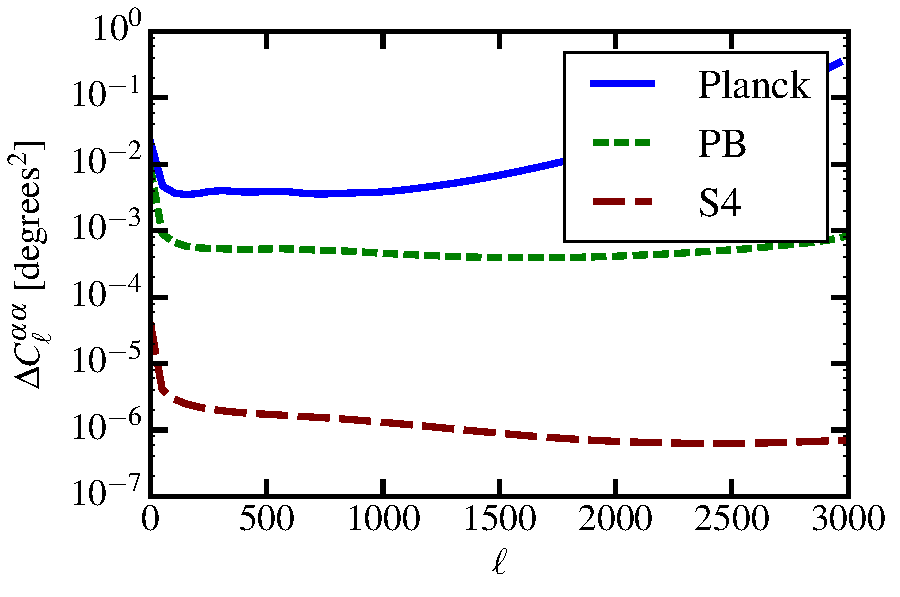
\includegraphics[width=0.70\textwidth]{BSMPhysics/birefringence-S4-planck-PB-v2.pdf}
\caption{The current (from POLARBEAR, labeled as PB) and projected (for Planck and Stage-IV experiment) 1$\sigma$ errobars on the birefringent rotation-angle power spectrum are shown on the vertical axis. A Stage-IV has the potential to improve the current best constraint on anisotropic birefringence by more than two orders of magnitude at all multipoles. For the Stage-IV forecast, we assumed noise of $1.41$ $\mu$K-arcmin (in polarization), a resolution of 1', and have considered polarization modes from $\ell=30$ to $\ell=5000$.}
\label{fig:CB-forecast}
\end{figure}

For a fixed integration time (and a varied noise level and sky coverage), large sky coverage optimizes sensitivity to low multipoles of the rotation angle and gives the best signal-to-noise ratio for rotation models that have power on large scales (such as, for example, a model with a scale-invariant power spectrum, which could result from fluctuations in a spectator scalar field present during inflation). Conversely, for models that have power on scales corresponding to multipoles above $\ell\sim 1000$, best signal-to-noise is achieved with deeper integration on small sky patches.  For a measurement of the magnitude of the quadrupole of the rotation angle, reducing the resolution from 1' to 9' produces a factor of a few increase in the projected errorbar (for all other parameters fixed). Increasing the noise from $1.41$ to $12.7$ $\mu$K-arcmin produces a factor of about $20$ increase in the errorbar. Access to polarization modes down to $\ell=2$ does not significantly affect the forecasts. 



